\textbf{Bluetooth Low Energy (BLE) Beacon} technology was utilized to accurately determine the user's location and provide them with relevant information regarding their current region and nearby points of interest. Furthermore, it was employed to notify the user if they are approaching a curve and indicate the appropriate direction to follow.

For this purpose was used the SDK provided directly by the beacon manufacturer and, through the information obtained with the latter, a localization logic was implemented, which was called \textbf{"region-based localization"}.

\begin{figure}[H]
    \centering
    
\includegraphics[scale=0.4]{chapters/architecture/images/beacon.jpg}
    \caption{Example of Kontakt iBeacon used to instrument the environment}
\end{figure}


\subsubsection{Kontakt SDK}
The SDK provided by \textbf{kontakt.io} was used to develop the Android application, integrating the localization logic for beacons through the methods it provides. \cite{kontakt:sdk}

Through the use of the \textbf{Proximity Manager}, a high-level component that allows to set the configuration information and scanning the devices, it was possible to receive information from the beacons. 
In particular, this component was able to provide information regarding newly discovered beacons and the signal update of already scanned beacons, returning the information needed to implement the localization logic, such as the \textbf{IDs} of the scanned beacons and their \textbf{Received Signal Strength Indicator (RSSI)}.


\subsubsection{Region-Based Localization\\ Method}
The \textbf{localization method} developed using BLE beacons divides the areas into regions, which are defined by the two beacons with the highest RSSI values.

The initial step entails uploading JSON files containing the required information regarding regions, points of interest, and curves. Moreover, the system consistently listens for incoming data from the beacons, extracting their IDs and RSSI values.

Whenever information is received from newly discovered or updated beacons, the system performs a check to determine if the two beacons with the highest power levels can form a new region. If the IDs of these beacons do not correspond to an existing region, the check is then extended to the next set of beacons. This process continues, iterating through all possible combinations of the three beacons with the highest power levels. By doing so, the search for a new region is optimized, ensuring that false positives are not created.

The transition from one region to another is determined by a predefined threshold. For a region to be recognized as the current region, it must be scanned a minimum number of times equal to the threshold value. Once the threshold is reached, the system considers the new region as the current one and triggers the transition accordingly. Whenever a region change occurs, the user is promptly notified of the current region, this notification includes a list of points of interest that are located within the newly identified region.

During region transitions, it is possible for a region to be identified as a \textbf{pre-curve} or a \textbf{curve}. When a region change occurs, the system checks if the current region is a pre-curve. If it is, the pre-curve ID is saved for future reference. On the other hand, if the current region is a curve, the system notifies the user about the upcoming turn. By utilizing the previously saved pre-curve ID, the system is able to determine the appropriate direction for the user to navigate while approaching the curve. This functionality ensures that the user receives timely alerts and guidance for navigating through curves and pre-curves.

\vspace{3mm}
\begin{figure}[H]
    \centering
    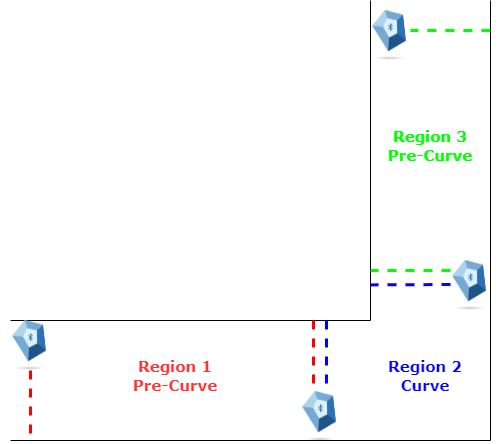
\includegraphics[width=0.9\columnwidth]{chapters/architecture/images/ble_beacons_regions.png}
    \caption{Example of environment region-based division delimited by 2 beacons}
\end{figure}
